%%%%%%%%%%%%%%%%%%%%%%%%%%%%%%%		APP		%%%%%%%%%%%%%%%%%%%%%%%%%%%%%%%

\chapter{Booster Neutrino Beam}
\label{app:A}

 Arxiv 1311.5958v1.
 Fermilab has two major neutrino beamlines: the Neutrino Main Injector (NuMI) and %
 the Booster Neutrino Beam (BNB).
 The energy range of these two neutrino sources on-axis is in the GeV range, %
 which is too high to satisfy the condition for dominance of coherent scattering. 
 The BNB source has substantial advantages over the NuMI beam source owing to suppressed %
 kaon production from the relatively low energy 8 GeV proton beam on the target~ref. 
 Therefore, pion decay and subsequent muon decay processes are the dominant sources of neutrinos. 
 At the far-off-axis area, the detector can be placed close enough to the target to gain a %
 large increase in neutrino flux due to the larger solid angle acceptance.
 Moreover, the far-off-axis (> $45^\circ$) of the BNB produces more defined neutrinos, with %
 energies below 50 MeV.

 The Booster is a 474-meter-circumference synchrotron operating at 15~Hz. 
 The beam is extracted into the BNB using a fast-rising kicker that extracts all of the particles %
 in a single turn: protons from the Fermilab LINAC are injected at 400 MeV and accelerated to 8~GeV kinetic energy, %
 or \np{8.89}~GeV/c momentum by the Booster.
 It has a harmonic number of 84, but the beam is structured in a series of 81 proton bunches %
 each 2~ns wide and 19~ns apart. 
 Upon leaving the Booster, the proton beam is transported through a lattice of focusing %
 and defocusing quadrupole (FODO) and dipole magnets.
 A switch magnet steers the beam to the main injector or to the BNB. 
 The BNB is also a FODO that terminates with a triplet that focuses the beamon the target. 
 The maximum allowable average repetition rate for delivery of protons to the BNB is %
 5~Hz (with a maximum of 11 pulses in a row at 15~Hz) and \np{5e12}~protons per pulse. 
 The 5~Hz limit is set by the design of the horn and its power supply.

 \section{The target}
 \label{sec:targ}

 %\begin{wrapfigure}{R}{0.5\textwidth}
 \begin{figure}[]
  \centering
  \includegraphics[scale=.2]{pics/target.png}
  \caption{An exploded view of the beryllium target assembly. 1) target base block; 2) bellow contact system; %
  3) upstream target slug locator and ring; 4) target slug, upstream; 5) target slug pin; 6) target slug, middle; %
  7) target slug, downstream; 8) air cool standoff; 9) window flange; 10) beryllium window; %
  11) base plug; 12) lock ring; 13) outer tube flange; 14) outer tube; 15) onstream target slug locater and gasket.}
  \label{fig:bnbtarget}
 %\end{wrapfigure}
 \end{figure}

 The target is made of beryllium divided in seven cylindrical sections in a total of \np{71.1}~cm, %
 in length, or about 1.7 inelastic interaction length, and \np{0.51}~cm in radius.
 The target is contained within a beryllium sleeve \np{0.9}~cm thick with an inner radius of \np{1.37}~cm.
 Each target slug is supported within the sleeve by three ``fins'' (also beryllium) %
 which extend radially out from the target to the sleeve.
 The volume of air within the sleeve is circulated to provide cooling for the target when the beam %
 line is in operation.
 An exploded view of the various components, with the downstream end of the target on the right, %
 is outlined in Fig.~\ref{fig:bnbtarget}.
 The choice of Be as the target material was motivated by residual radioactivity issues %
 in the event that the target assembly needed to be replaced, as well as energy loss %
 considerations that allow the air-cooling system to be sufficient.
 The vacuum of the beam pipe extends to about 150 centimetres upstream of the target, %
 minimizing upstream proton interactions.

 \section{The Horn}
 \label{sec:horn}

 \begin{wrapfigure}{R}{0.5\textwidth}
 %\begin{figure}[]
  \centering
  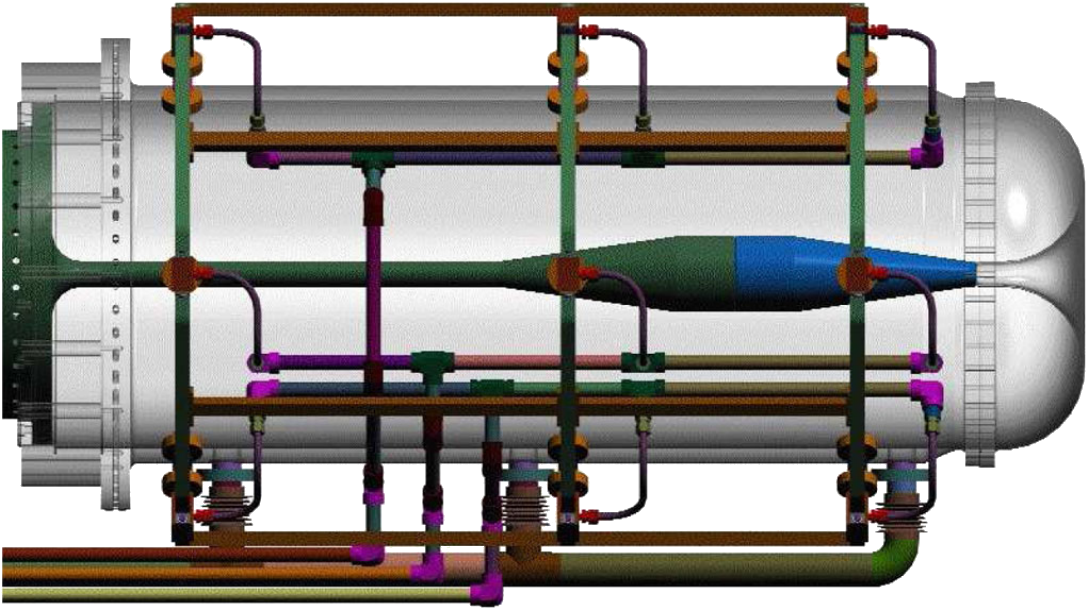
\includegraphics[scale=.2]{pics/bnbhorn}
  \caption{BNB horn system.}
  \label{fig:bnbhorn}
 \end{wrapfigure}
 %\end{figure}

 The horn, shown in Fig.~\ref{fig:bnbhorn}, is a pulsed toroidal electromagnet composed of an aluminum %
 alloy (6061 T6), which surrounds the target.
 This device bends, sign-selects, and focuses the secondary particles that emerge from the interactions %
 in the beryllium, along the direction pointing to the detector.
 The current flowing in the horn is a 143~$\mu$s-long pulse half sinusoid, with a nominal amplitude of 170~kA %
 coinciding with the arrival of the proton beam at the target.
 The actual operating values are typically 174~kA in both neutrino mode (positive current) and antineutrino mode %
 (negative current), with \np{+-1}~kA variations.
 In neutrino mode, the flow of current runs along the inner conductor, which folds outwards at a length of %
 185~cm to return via the outer conducting cylinder of the horn at 30~cm radius.
 Within the horn cavity, defined by the volume between the outer and inner conducting cylinders, %
 the pulse creates a magnetic field that falls as $1/R$, where $R$ is the distance from the cylindrical symmetry %
 axis of the horn.
 The largest magnetic field values of \np{1.5}~T are obtained where the inner conductor is narrowest %
 (\np{2.2}~cm radius).
 The ``skin effect'', in which the time-varying currents traveling on the surface of the conductor penetrate %
 into the conductor, results in electromagnetic fields within the conductor itself.
 However, the effects of time-varying fields within the cavity of the horn are found to be negligible.
 The target assembly is rigidly fixed to the upstream face of the horn, although the target is %
 electrically isolated from its current path.

 A concrete collimator is located downstream of the target and guides the beam into the decay region.
 The air-filled cylindrical decay region extends for 45~m, 90~cm radius. 
 The beam stop is made of steel and concrete. 
 The beam of focused, secondary mesons emerging from the target/horn region is further collimated, %
 via passive shielding, and allowed to decay into neutrinos in a cylindrical decay %
 region filled with air at atmospheric pressure, 50 m long and 90 cm in radius. 
 A beam absorber located at the end of the decay region stops the hadronic and muonic %
 component of the beam, and only a pure neutrino beam pointing toward the detector remains, %
 mostly from a pion to mu+ nuofmu decays.

 \section{Monitoring}
 \label{sec:monitor}

 Upstream of the target, the primary proton beam is monitored using four systems: %
 \begin{itemize}
   \item two toroids measuring its intensity (protons per pulse);
   \item beam position monitors (BPM);
   \item a multiwire chamber, that in combination with the BPMs determines the width and position of the beam;
   \item a resistive wall monitor (RWM) measuring both the time and intensity of the beam spills.
 \end{itemize}

 The number of protons delivered to the BNB target is measured for each proton %
 batch using the toroids located near the target along the beam line. 
 The toroids are continuously calibrated at 5~Hz with their absolute calibrations verified %
 twice a year.
 The calibrations have shown minimal deviation (< \np{0.5}\,\%).
 The proton flux measured in the two toroids agree to within 2\%, compatible with the %
 expected systematic uncertainties.

 The BPMs are split-plate devices that measure the difference of charge induced on two plates. 
 By measuring the change in beam position at several locations without intervening optics, %
 the BPMs are found to be accurate to \np{0.1}~mm.
 The typical beam alignment and divergence measured by the beam profile monitors located %
 near the target are within 1~mm and 1~mrad of the nominal target center and axis direction, %
 respectively.
 These parameters are well within the experiment requirements. 
 The multiwire is a wire chamber with 48 horizontal and 48 vertical wires and \np{0.5}~mm pitch. 
 The profile of the beam is measured using the secondary emission induced by the beam on the wires.

 The RWM is located upstream of the target to monitor the time and intensity of the proton %
 pulses prior to hitting the target, by measuring the image charge that flows along the vacuum %
 chamber following the beam.
 The image charge has equal magnitude but opposite sign and in order to measure it, the beam pipe is cut %
 and a resistive gap is inserted. 
 Depending on the beam velocity, the image charge will lag behind and be spread out along its path. 
 The ultimate bandwidth of such a detector is limited by this spreading of %
 the electric field lines between the beam and the inside walls of the beam pipe.
 Various ferrite cores are used to force the image current through the resistive gap rather %
 than allowing it to flow through other conducting paths.
